\documentclass[12pt, a4paper]{article}
\usepackage[utf8]{inputenc}
\usepackage{formatting}



\begin{document}

\thispagestyle{empty}

\vspace*{-1.5cm}

\noindent \textit{2024 - pt-br}

\vspace*{14pt}
{
\fontsize{32pt}{24pt}\selectfont{
    \begin{center} \bfseries{ {Guia Monitor PSoC 6}} \end{center}
	}
}
\vspace*{12pt}

\tableofcontents

\section{Montagem do Experimento}

Esta parte do guia visa mostrar o passo a passo para a montagem do experimento com Neutrons utilizando o PSoC 6.

\addcontentsline{toc}{subsection}{Pré-requisitos}
\subsection*{Pré-requisitos}

\begin{itemize}[leftmargin=1.3cm]
    \item Certifique-se que o sistema operacional não será suspenso ou desligado automaticamente nas opções de energia do computador;
    \item Obtenha o software \text{"monitor\_psoc"} para o sistema operacional escolhido;
    \item Tenha em mãos os dois kits de desenvolvimento e os cabos USB para a conexão dos dispositivos com a interface serial do software.
\end{itemize}

\begin{figure}[H]
    \centering
    \caption{(DUT) - Kit de Desenvolvimento Infineon CY8CPROTO-063-BLE}
    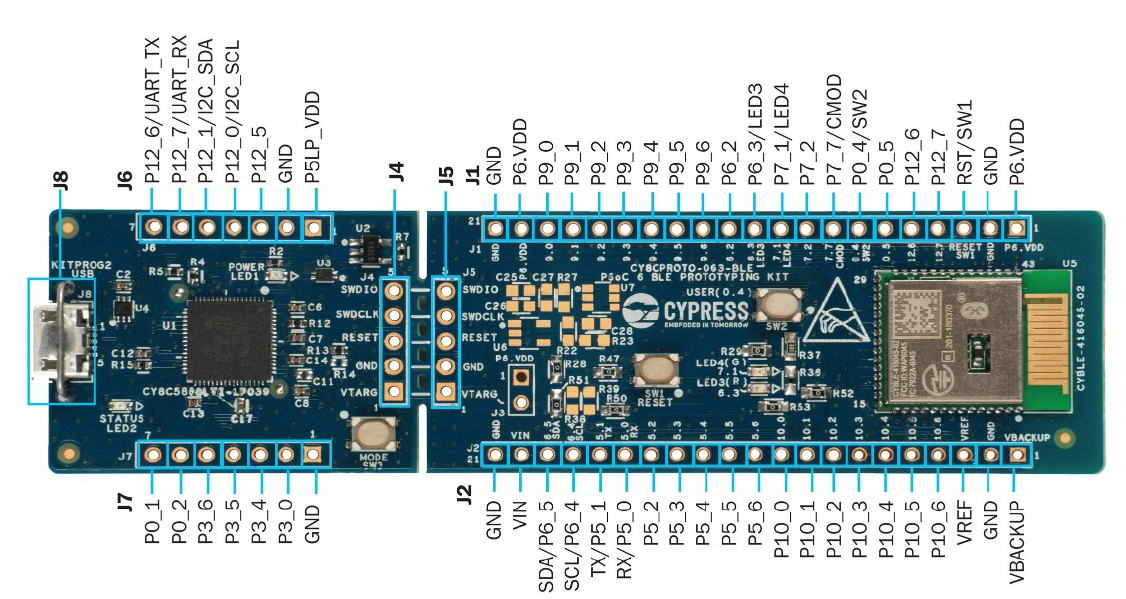
\includegraphics[width=0.5\textwidth]{../imgs/psoc63_DUT.png}

    \vspace{0.5em}
    \label{fig:psoc6}
\end{figure}

\begin{figure}[H]
    \centering
    \caption{Watchdog - Kit de Desenvolvimento Infineon CY8CPROTO-062-4343W}
    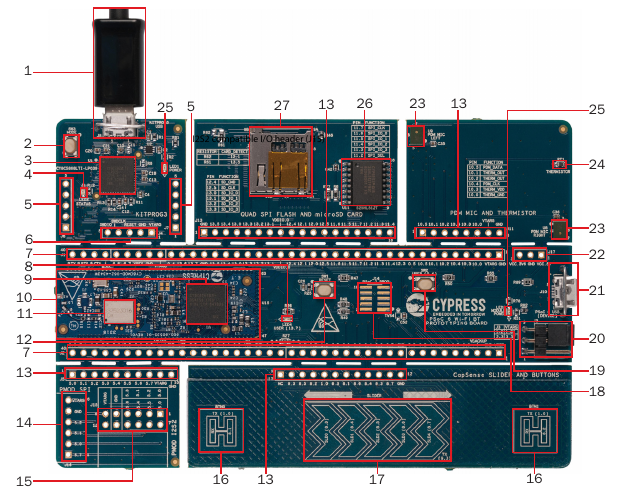
\includegraphics[width=0.5\textwidth]{../imgs/psoc62_watchdog.png}

    \vspace{0.5em}
    \label{fig:watchdog}
\end{figure}

\addcontentsline{toc}{subsection}{Etapas}
\subsection*{Etapas}

\begin{enumerate}[leftmargin=1.3cm]
    \item  Realize a conexão das placas conforme está representado no diagrama da figura abaixo:
\end{enumerate}

\begin{figure}[H]
    \centering
    \caption{Esquema de conexões para o experimento}
    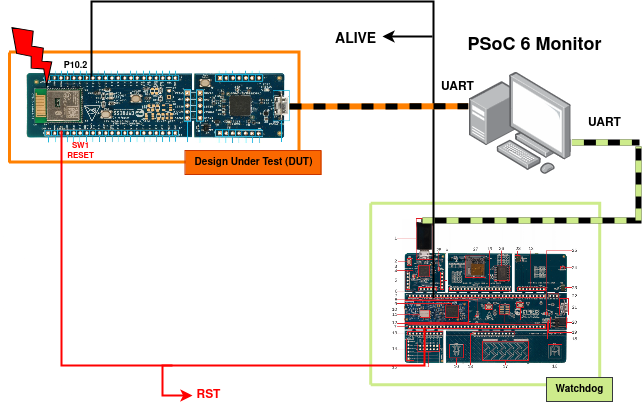
\includegraphics[width=0.8\textwidth]{../imgs/esquema_ligacoes.png}

    \vspace{0.5em}
    \label{fig:diagrama_con}
\end{figure}

\begin{enumerate}[leftmargin=1.3cm]
    \setcounter{enumi}{1}
    \item  Abra o software de monitoramento, entre em ``Start Monitoring" e escolha a porta serial que cada dispositivo está conectado.
\end{enumerate}

Para descobrir a porta serial dos dipositivos, o usuário poderá entrar em Gerenciador de Dispositivos no windows coforme a figura abaixo:

\begin{figure}[H]
    \centering
    \caption{Windows - Gerenciador de dispositivos}
    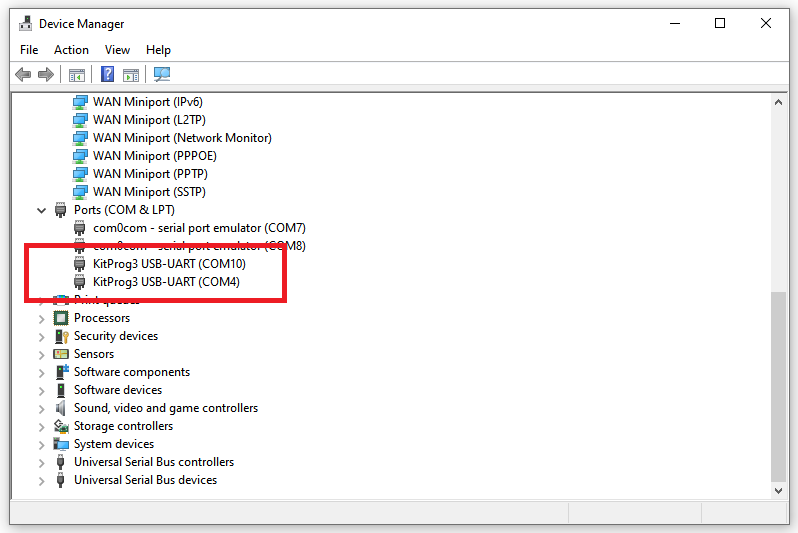
\includegraphics[width=0.7\textwidth]{../imgs/device_manager.png}

    \vspace{0.5em}
    \label{fig:device_manager}
\end{figure}

Ou então, se o sistema operacional for linux, listar as portas utlizando: ``ls /dev/ttyUSB* /dev/ttyACM*". Caso o usuário tente conectar o kit errado, o software acusará "Error connecting to port!" após de "Attempting connection \text{...}" e então basta selecionar a outra porta serial.

\begin{figure}[H]
    \centering
    \caption{Conectando portas seriais no Linux}
    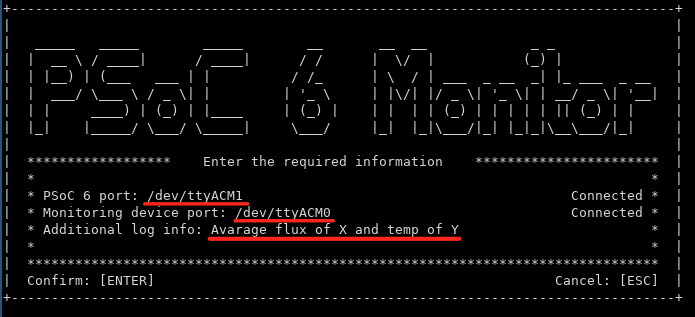
\includegraphics[width=0.8\textwidth]{../imgs/serial_linux.png}

    \vspace{0.5em}
    \label{fig:serial_linux}
\end{figure}

\begin{enumerate}[leftmargin=1.3cm]
    \setcounter{enumi}{2}
    \item Adicione informações sobre o experimento em ``Additional log info" como o fluxo de neutrons escolhido ou a temperatura do local. Essa informação será adicionada ao cabeçalho do arquivo de log da sessão iniciada.

    \item Verifique se o experimento está sendo executado corretamente:
\end{enumerate}

Ambos os kits devem ter seus leds piscando (watchdog vermelho e DUT verde) que proporcionam uma indicação visual que o processamento está sendo realizado de acordo. Já o software de monitoramento deverá se assemelhar inicialmente ao da figura abaixo, com ambos aparelhos ``Connected", número de buffers recebidos e resets zerados. 

\begin{figure}[H]
    \centering
    \caption{Menu de monitoramento}
    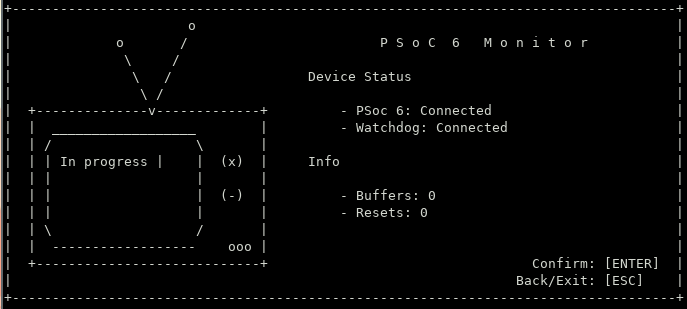
\includegraphics[width=0.8\textwidth]{../imgs/monitoring.png}

    \vspace{0.5em}
    \label{fig:monitoring_menu}
\end{figure}

\begin{enumerate}[leftmargin=1.3cm]
    \setcounter{enumi}{3}

    \item Registre uma foto da montagem do exemperimento para ser encaminhado juntamente com os arquivos \text{.}log.

    \item Para finalizar a sessão de monitoramento corretamente, o usuário deve apertar ``ESC" e após confirmar com ``ENTER" \text{.} Feito isso, será adicionado ao final do arquivo de log um resumo da sessão com todos os dados obtidos. 
\end{enumerate}

\section{Atualizando o Firmware}

Caso seja necessário regravar a imagem da flash do dispositivo, o usuário -- com o arquivo \text{.}hex em mãos -- pode utilizar o programa PSoC Programmer que é encontrado para windows pelo link: https://softwaretools.infineon.com/tools/com.ifx.tb.tool.psocprogrammer

% Image PSoc Programmer

O passo a passo de como carregar o arquivo para o SOC é explicado no seguinte vídeo: https://www.youtube.com/watch?v=aPe2A1J0OIA
\end{document}

